\null\newpage
\section{Tieftöner-Verstärker}\label{sec:4.4}
\subsection{Allgemeines}\label{subsec:4.4.1}
Nach dem Filtern des Signals soll dieses vor dem Abstrahlen am Lautsprecher verstärkt werden. Es wurde eine analoge Verstärker-Schaltung verwendet, da diese einfacher und mit weniger Problemen realisiert werden konnte. Mithilfe bereits bekannter, bewährter Schaltungen konnte ein Layout für diese Schaltung designet werden. Ein wichtiger Baustein in dieser Schaltung ist der Verstärker \enquote{TDA2030}, wie in Kapitel \ref{sec:3.2} beschrieben.  Des weiteren wurden zwei Leistungstransistoren verbaut die höhere Ströme schalten können, falls der maximale Schaltstrom des TDA2030 erreicht wird.

\subsection{Zielsetzung}\label{subsec:4.4.2}
Das Eingangssignal soll verstärkt werden um am Ausgang der Schaltung höhere Spannungs-Amplituden und höheren Ströme aufzuweisen. Es soll nach diesem Schritt möglich sein den Tieftöner in einer der zwei Satellitenboxen mit ausreichend Signal zu versorgen, um einen Schalldruck von zumindest Zimmerlautstärke zu erhalten. 

\subsection{Schaltung}\label{subsec:4.4.3}
Leicht ersichtlich in der Schaltung (\ref{fig:4.4.4.1}) ist in der oberen, linken Ecke des Bildes ein Spannungsteiler gegen den Einseranschluss des TDA2030.
Dieser Spannungsteiler, bestehend aus einem Widerstandsnetzwerk, erzeugt den benötigten Arbeitspunkt für die asymmetrische Versorgung des TDA2030.
Mit Hilfe des ELKO's \enquote{EL504} wird verschleppte Gleichspannung am Eingang der Schaltung heraus gesiebt.
Dafür ist auch der ELKO \enquote{EL502}, dieser siebt die Gleichspannung am Ausgang der Schaltung heraus, bevor das Signal den Print verlässt. \\
Über die Widerstände \enquote{R506} und \enquote{R505} wird die Verstärkung der Schaltung eingestellt.
In diesem Fall ist die Verstärkung $\frac{R505+R506}{R505}$ = 31 .
Das bedeutet, dass das Eingangssignal am Ausgang 31mal so groß sein soll, natürlich unter Beachtung der Grenzen der OPV-Verstärkerschaltung(\ref{sec:3.5}).

\begin{figure} [H]
	\centering	
	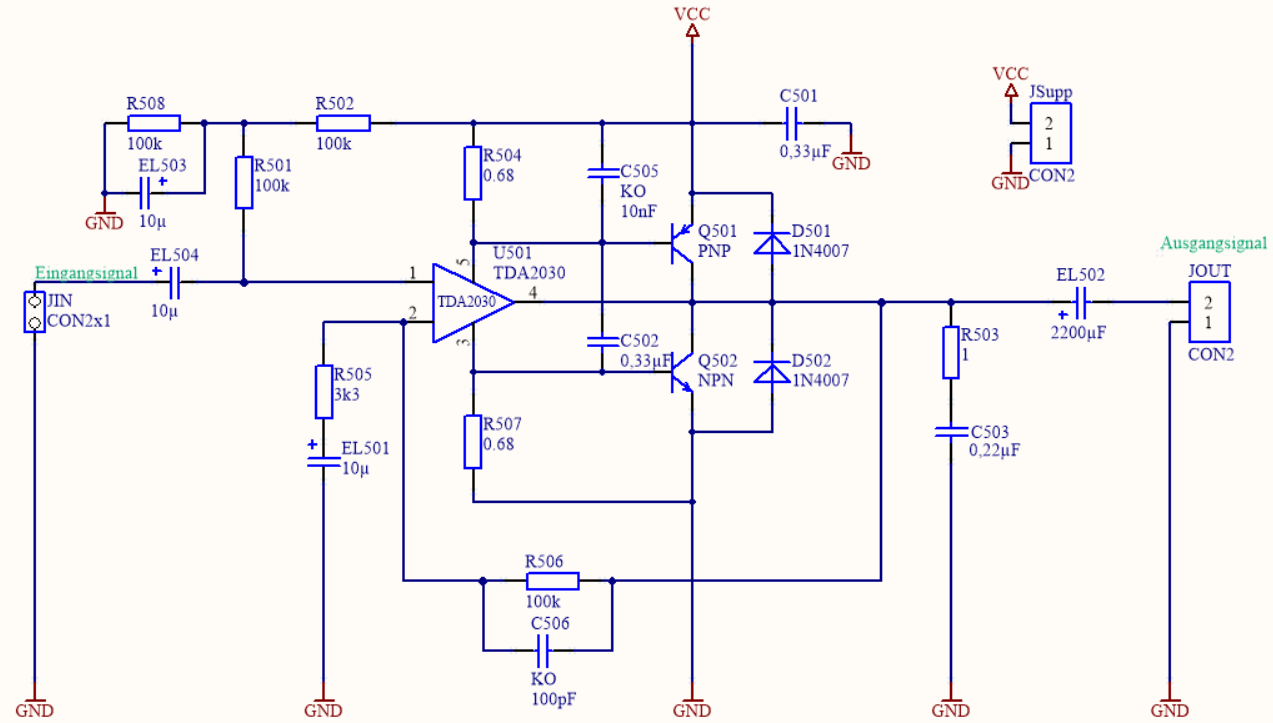
\includegraphics[width=1\textwidth]{img/Print5/5_TTVerstaerker-Schem.PNG}
	\caption{Tieftöner-Verstärker Schaltung}
	\label {fig:4.4.4.1}
\end{figure}